%!TEX root = project.tex

\chapter*{About this project}
\paragraph{Abstract}
The aim of this project is to allow users the ability to have a user friendly bitcoin wallet to store their bitcoins. We want to have a sercue wallet that allows the users to register and log in to the application with their information safely storing to a database. 

\paragraph{Authors}
Explain here who the authors are.



\chapter{Introduction}
This chapter will outline the objectives of the project along with the scope which we plan to complete those objectives in. An analysis of each of the chapters found in this dissertation along with a summary Github repository containing the project can be found below. This application will aim to satisfy the standards for a Software Development Level 8 project by surpassing the expectation of cryptocurrency wallets currently offered online. Bitcoin has received vast media coverage in the recent months because of its record high price. This brought a lot of new attention towards the technology, but to invest in or use this decentralized currency a benchmark of software and economic knowledge must be met. The members of this group have taken it upon themselves to create an application that not only allows users to use the cryptocurrency in a practical sense, but will also educate the users about the coins and offer feature relevant to members of the bitcoin community. Proper authentication and login will be applied to the app to allowing users to easily assess there coins securely and associate relevant information to an address that will be stored in a NoSql database. Most of the technologies discussed here are emerging technologies that are not taught in the Software Development in GMIT.

\subsection{Objectives:}
\begin{itemize}
  \item Make the UI user friendly and appealing to new users of Bitcoin.
  \item Educate user on the technology bitcoin and how it works, display real time value.
  \item Strong authentication that’s simple to use yet secure so users will trust us with their coins.
  \item Google Maps integration to show users bitcoin related locations like exchanges or stores that accept the currency.
  \item Use QR codes to easily send and receive coins.
\end{itemize}

\section{Specifications}
\subsection{Web application:}
\begin{itemize}
  \item Receive bitcoin from external wallets at any time.
  \item Send bitcoin to external wallets at a fast and efficient rate using.
  \item Allow users to see their balance displayed clear and aesthetically.
  \item Google maps page show related bitcoin locations.
  \item Bitcoin price display showing the current value and related stats.
  \item Create new user.
  \item Log in.
  \item Log out.
  \item Update user details.
  \item QR Code integration.
  \item Delete user.
  \item Display related bitcoin news.
  \item Information pages to educate different bitcoin userst.
\end{itemize}

\subsection{Database:}
\begin{itemize}
  \item Should store user details.
  \item Should store bitcoin address.
  \item Should store contacts.
\end{itemize}

\subsection{Server:}
\begin{itemize}
  \item Provide secure routes for users.
  \item Authenticate users.
  \item Send requests received from web app to database.
  \item Receive and forward database responses to web app.
\end{itemize}


\subsection{The rise of the first cryptocurrency}
On the October 31, 2008 by a computer scientist, programmer or group of programmers under the name of Satoshi Nakamoto published the first digital currency also know as the first 'cryptocurrency'. This technology attracted the attention of many because of its decentralization, meaning governments or organizations could not intervene with the blockchains distribution of bitcoins or control the currency that is bitcoin. Satoshi Nakamoto also published a research paper titled \cite{Satoshi}'Bitcoin: A Peer-to-Peer Electronic Cash System' that explained how the system operates and functions. It explained how the miners power the system by solving a complicated mathematical equation using an input provided by the previous block and an input provided by the miners CPU. The miners would then announce the solution to the rest of the network so other miners could validate the new block and assuring the blockchains integrity. Users of bitcoin did not have to rely on outside intervention from a 3rd party for their online transactions as this mathematical proof-of-work approach eliminated the need for each person involved to give their identities to the 3rd party, allowing them to send bitcoin to other addresses or freely exchange bitcoin for goods and services and allowing the exchange of value to be taken care off by the system.

\subsection{Bitcoin: What is a bitcoin?}
A bitcoin can be thought of as a digital receipt, its really a list of locations starting at the block that generated the coin. Currently when a block is solved the miner is rewarded with a transaction fee collected from each transaction within the block along with newly generated bitcoin. This is the start of a bitcoins lifespan and each new address the bitcoin gets sent after being generated will be recorded. Validation of the bitcoins history and location are done using a private key and public key. When someone sends a bitcoins from one address to another the user uses their public and private key to sign the transaction and then the receiver of the bitcoins compares the public key to the address listed on the transaction. Once everything is in place the transaction is placed in a block to be validated on the blockchain. If this process was to be repesented as a design pattern it would look like the following.

\begin{figure}[H]
\centering
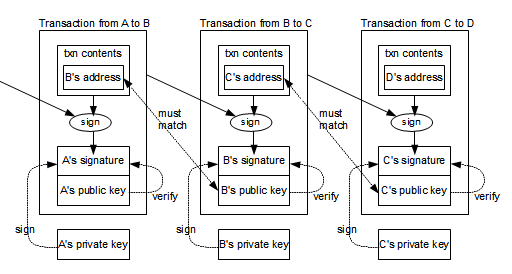
\includegraphics[scale=0.55]{img/bitcoindesign.png}
\caption{Design pattern.}
\end{figure}

If we where to represent a bitcoin as a design pattern like the above and included the first transaction of a bitcoin from the address that generated the value all the way to the most recent exchange from the previous address to the current address would be a good representation of what a bitcoin looks like. Representing value in this digital record approach appeals to many as it doesn't require overhead administration  to work along with no enforcing of policy's or rules of use by an administrator. There is no physical copy of the value meaning it is a lot harder to steal or go missing, it also does not take up space in the physical world. No validating of the exchange by a 3rd party or outside source means transactions can be a lot faster compared to there fiat counterpart. The autonomous method for creating bitcoins at a set rate until a certain amount exist gives a scarcity and value to the coin as more cannot be printed.

\subsection{Blockchain: What is the blockchain?}
The block-chain is a design pattern that came about with the creation of bitcoin, this design pattern solved a problem that plagued computer scientists during the early years of the internet. The problem was how can we have people exchange services and things of value on the internet without a middleman or overseeing power having to get involved. The blockchain works by combining the collective processing power of computer systems worldwide in order to process transactions. These machines vary from high performance computers to groups of less effective computers known as mining pools. About every 10 minutes these computers, also known to the cryptocurrancy community as "miners" will collect a bunch of pending transactions and create a unsolved block. To solve the block we take the address of the previous block and combine it with a nonce which is provided by the miner’s CPU power, this this is just a newly generated hash similar to the one from the previous block. Saoshi mentions in the published paper that the two hash strings are used in a series of calculations based on Adam Back's Hashcash, a algorithm created to stop denial-of-service attacks using cryptographic hashes such as SHA1, SHA256 or SHA3. The hash that is taken as the solution is the first miner to produce a SHA256 hash that has a header starting with a specified number of 0’s set by the block-chains difficulty.  The block-chain difficulty fluctuates depending on the rate of blocks being produced. Below is a simplified representation of what the blockchain looks like.
\begin{figure}[H]
\centering
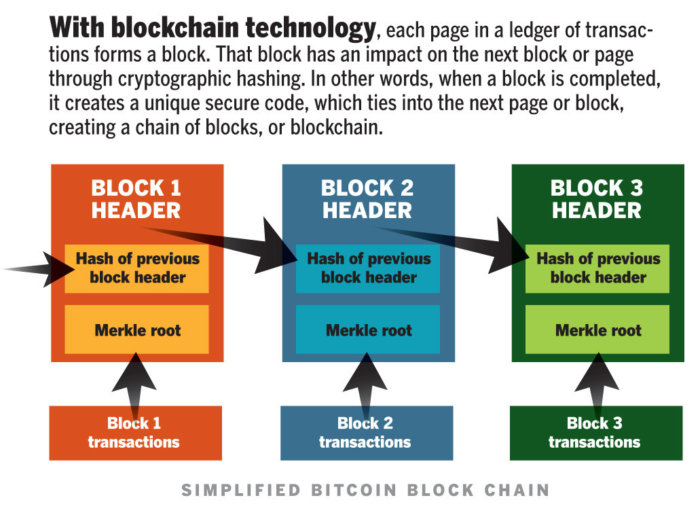
\includegraphics[scale=0.5]{img/blockchaindesign.jpg}
\caption{Blockchain.}
\end{figure}
\subsection{Applications interactions with the blockchain: API's}
\textbf{Blockchain.info:} This is a website that can be used to examine transactions and blocks that have been validated on the blockchain. You can also use this site to create an online wallet for storing your own bitcoins. You can apply for an API which will grant you the ability to integrate the blockchain into your application allowing you to create a wallet, send and receive bitcoins and get information on transactions. The API uses POST and GET calls to return JSON to the application which can be then used. \break
\textbf{BlockCypher:} This is another API that returns JSON to the application. BlockCypher is for interacting with blockchains, accessed over HTTP or HTTPS from the api.blockcypher.com domain. One of the major pros of using this service is that it does not only offer just the bitcoin blockchain but also Ethereum, Litecoin and Dogecoin. \break
\textbf{Coinbase API:} This API is offered by the one of the most popular exchanges coinbase. This is a well established site with an API that allows you to create wallets along with sending and receiving bitcoin. This API allows you to add widgets to your application allowing users to buy bitcoin.

\chapter{Context}
\begin{itemize}
\item Provide a context for your project.
\item Set out the objectives of the project
\item Briefly list each chapter / section and provide a 1-2 line description of what each section contains.
\item List the resource URL (GitHub address) for the project and provide a brief list of the main elements at the URL.
\end{itemize}

\section{Filler}


\subsection{More filler}


\section{Filler}



\chapter{Methodology}
About one to two pages.
Describe the way you went about your project:
\begin{itemize}
\item Agile / incremental and iterative approach to development. Planning, meetings.
\item What about validation and testing? Junit or some other framework.
\item If team based, did you use GitHub during the development process.
\item Selection criteria for algorithms, languages, platforms and technolo-gies.
\end{itemize}
Check out the nice graphs in Figure \ref{tikz:graphs}, and the nice diagram in Figure \ref{tikz:mydiagram}.

\section{Platform Design}

As a group Conor, Donal and I(Stephen) met regularly each week and our first plan of action was to divide the work and objectives between the 3 of us. I offered to take on some of the front end and the primary load of the aesthetics/ overall look of the project. I had previous experience in graphic design so I photo-shopped mock designs and thumbnails for the project as we went on. I familiarized myself with how the mean stack controlled its colour scheme and look through bootstrap, CSS and HTML components. I researched a lot of different style-sheets and components to make the projects UI(user interface) stand out and be intuitive. I had working design in my head that I wanted to achieve, along with receiving creative input form Conor and Donal.

I started with the aesthetic of the home page first. Making a 2 by 2 grid with 4 thumbnails that linked to different components of the project. To make this grid and to centre it I used a CSS sheet for the home component HTML page. I wanted each of these thumbnails highlight when hovered on and portray exactly what they linked to. To do so I used Adobe Photoshop for editing and graphic design. For inspiration and templates/base images I used Google images with key words to find exactly what I was looking for. I looked at various crypto-currencies wallets, stock websites and angular apps to get a feel for how this project should look. I want to take the best aspects from each and improve on areas where I felt these other platforms could have. 

Conor informed me about Google fonts. Google fonts is a font hub offered by Google offering a free download of a endless amount of varying fonts. I browsed through the website and found multiple fonts I felt would fit the idea for the look of the app. 
My criteria for picking a font was



\chapter{Technology Review}
About seven to ten pages.
\subsection{MEAN}
the following four technologies are the fundamentals of a MEAN stack(Mongodb,Express,Angular,NodeJS).

\subsection{Mongodb:}
MongoDB is a free, open source cross-platform database program. It is
document-oriented which means it is designed for storing, retrieving, and
managing document-orientated information. This is also known as semi
structured data. MongoDB is a NoSQL database program and uses JSONlike
documents with schemas. MongoDB is a distributed database and is
designed for ease of development and scaling it also possesses satisfying scalability
and flexibility. The document model maps to the objects in your application
code which makes data easy to work with. Ad hoc queries, indexing,
and real time aggregation provide powerful ways to access and analyse your
data\cite{WhatIsMo75}.
\\
MongoDB provides a wide range of beneficial features for users. For file
storage, large objects or files are easily stored within MongoDB. MongoDB
supports an easy to use protocol for storing large files and files metadata. Incredible
performance is a major goal for MongoDB and has therefore shaped
much of its design\cite{usuarist10}.

\subsection{Angular2/5:}
This is a Typescript framework for JavaScript and HTML that was developed by Google. We built our front-end using Angular2 by using creating Angular components to represent part of HTML that can be served dynamically resulting in a high performance and reliable UI, any version of angular can be used with the MEAN stack but we decided to use Angular2 as it offers new features since the first version. Angular2/5 is a complete framework and is not to be confused with its predecessor AngularJS a JavaScript library.

\subsection{ExpressJs:}
This is a web application framework used by NodeJS that allows JavaScript to communicate with a database, this is what we will be using to get the data in out app from the front-end to the database.

\subsection{NodeJS:}
This is a run time environment for executing server-side JavaScript. This allows us to easily install libraries and add-ons using the node package manager with the command line.

\section{Other Technologies}

\subsection{Docker:}
Docker allows developers to use containers to ship and deploy there applications to system and users worldwide without having to worry about performance varying from each individual operating system or machine that the application runs on. A container can be thought of as a small virtual machine with a low resource demand that allows the application to run in a environment it has been tested and trialed on allowing the application to run in a optimized state and reducing the chances of software bugs and errors appearing.

\subsection{Github:}
GitHub is a web-based Git or version control repository and Internet hosting
service that was founded in 2008. GitHub provides both public and private repositories which are used to host open-source software projects. Public repositories are free to use but private repositories come at a fixed monthly cost. GitHub also provides a graphical user interface for
Windows and Mac, GitHub Desktop App to help eliminate the use of the command line tools for managing project uploads and commits, but many others prefer using the command line tool Git for this. In addition to code, Github supports the following formats and features: Documentation, issue tracking, wikis, graphs, integration directories, email notification and PDF document viewer\cite{WhatIsGi4}.
\\
Some sample git commands used are as follows:
\begin{itemize}
    \item git clone path/to/repo\par
    This command allows to clone any project from your github account
    or any publicly available project for that matter.

    \item git clone path/to/repo\par
    This command allows to clone any project from your github account
    or any publicly available project for that matter.
    
    \item git status\par
    Checks the status of project once it has been cloned it shows
    added deleted and modifies files as well as indicates which files
    are tracked.
    
    \item git add .\par
    Add folders or files to be tracked by github so later they can be
    committed and pushed on to github account.
    
    \item git commit –a\par
    Makes local commit of all the changes done in folder added by
    previous command git add .
    
    \item git push origin master\par
    Pushes commit (git commit -a) to users github account on his/her
    account
    
    \item git push origin +'COMMIT ID':master\par
    Reverts back to the state of the repo at the desired commit
\end{itemize}

\subsection{Bootstrap:}
Bootstrap is an open-source front-end framework which allows users to generate efficient UI components fast. We decided to use Bootstrap as it lets us create a dynamic application UI that will work on mobile, tablets, desktop etc.

\subsection{Blockchain:}
This application will be closely tied to the bitcoin blockchain, a technology created by an individual or group called Satoshi Nakamoto. we will use an API to directly interacted with this decentralized public ledger allowing users to recieve and send bitcoin from the application.

\subsection{Adobe Photoshop:}
Adobe Photoshop is a photo editor developed by Adobe System for Mac and Windows operating systems. Its initial release was in 1990. Adobe Photoshop is the premier photo editor used all over the world by graphic designers. From small one man teams to huge corporations Photoshop is prolifically used. This is why I chose Photoshop when choosing something to give a custom aesthetic to our application. Photoshop offers a dynamic way to customize the looks of the icons, thumbnails and profile pictures. 

\subsection{Google Fonts:}
Google Fonts is a font library API that offers over eight hundred fonts for use. It is also a interactive website that is easily browsed for finding the right font for your application or website. It helps create a dynamic UI and works across multiple platforms from mobile devices, desktop and many other devices.

\section{JavaScript}
JavaScript is a high-level, dynamic, programming language widely used alongside HTML and CSS employed by the majority of websites and supported by all modern web browsers. It is a small and lightweight language. It contains a standard library of objects, such as Date, Array, and Math and a core set of language elements such as operators, control structures, and statements\cite{Introduc25}.
The following is an example of JavaScript\cite{JavaScri59}:
\begin{lstlisting}
// Function is called, return value will end up in x
var x = myFunction(4, 3);   
// Function returns the product of a and b
function myFunction(a, b) {
    return a * b;   
}
\end{lstlisting}


\section{Social Media Research}

Social media plays a crucial part in our everyday lives. Whether we like to give it that much importance it is the most prominent and hugely influential factors in our world right now. Whole business have been set up and run off the back off these social media platforms, with new revenue streams being offered thanks to their existence. More and more each day people are dependant on social media for their news instead of news outlets which then informs the users views on certain topics and products. A products reception on the social media giants like Twitter or Facebook can be make or break. A couple bad tweets, posts on Facebook or rants on YouTube can result in PR nightmares for companies and loss in revenue and stock. Social media can also be used to document users trends and habits giving vital information on what the user wants to see and where the platform is heading. 
Facebook and Twitters ability to document users information and habits has helped them stay on top and stick with whats trending and not fall by the way side like many other social media platforms. This also leads to targeted advertisements a users search history and likes and viewings are used to inform what else they will see on a platform. For example a common thing you may have come across is: you have searched or liked something relating to a particular television show then you open up Instagram and scroll and the first advert that pops up is merchandise relating to that television show. This happens every day and with social media AI being trained to handle your own social sphere better and better your platform and overall experience can wind up completely different to those around you. 

So taking of this into account and to bring a educational crypto-currency platform to the market it is necessary to research the information and trends out there in the market and on social media. As discussed previously Social Media influences the market. Public opinion will influence the success of your product and in this day and age social media is public opinion. To Launch any sort of app these days, there Has to be some sort of social media interaction or built in functionality. Every app these days lets you follow your friends and informs you what they are doing. Each app has a communication/messaging service between its users. FAQ services and support between the user and the developer is of the up most importance a lot of this is done through social media. Take air line's social medias often people can complain to these accounts and the issues will instantly be resolved. No company wants a negative image on social media as they know people will be swayed. 

Public opinion on the topic that informs the app or the platform is based on is also hugely important. Taking this into account we can't just observe how our platform is interacts with social media and what people say about it on social media. We in fact have to look at the subject matter of our application, Bitcoin a violate crypto currency that everyone in the past year has an opinion on and has been talking about. Social media can literally affect the price of any crypto currency. From celebrities and social media personalities talking about and announcing their support or investment into a currency to people talking about the negative affects or downside of Crypto-Currencies. Bitcoin and Crypto-Currencies are a new wave and almost controversial topic. The information is out there but people aren't very well informed on the topic. With differing opinions and news flooding in on social media platforms it gets very confusing for the average person to know who to listen to and what to follow..


\chapter{System Design}
In this section, we will cover the overall design and implementation of the application with help from screenshots, code snippets and a UML diagram to visualize the structure.

\section{User Registration}

\subsection{Overview}
The user can register and create an account with the application through the register page. The register page is accessible through the opening page of the application by pressing the register button. This will bring you to the register page and will ask you for the necessary details in order to create an account. The information that's needed to create an account are as follows:
Username, Email address, Password and user will be asked to reenter their password to confirm it. The user must provide this information and it is then stored to our MongoDB database. When the users password is stored to MongoDB, their password is encrypted to make the application more secure. The users information that is stored to MongoDB can then be used to Login to the application. Below is a sample of the Registration interface and user information stored in MongoDB which is being viewed through Robo 3T.
\begin{figure}[H]
\centering
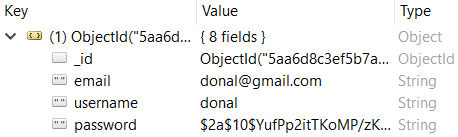
\includegraphics[]{img/UserInfo.png}
\caption{Data stored in MongoDB.}
\end{figure}

\begin{figure}[H]
\centering
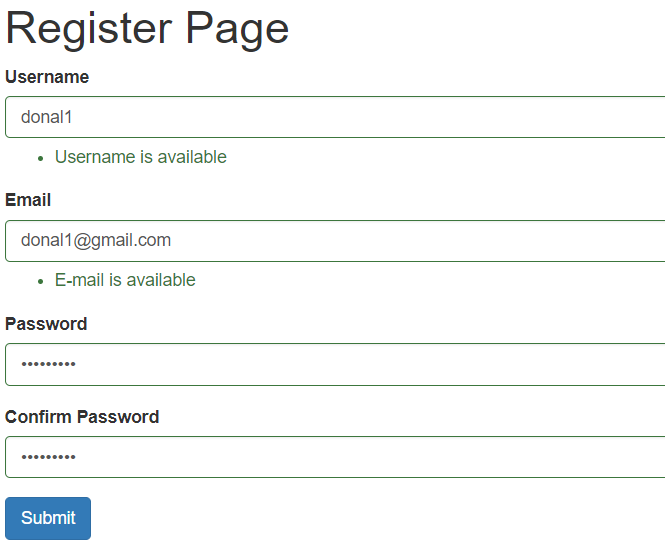
\includegraphics[]{img/UserInterface.png}
\caption{Registration interface.}
\end{figure}


\subsection{In-depth}
In the HTML of the register page, I created inputs that take a type text for the users username, email address, password and confirmed password. The submit button is unusable until the user has entered all the correct information. I have ngIf statements that give back errors or success information when the user is entering information. For example if a username is already taken, the application will return and tell the user that this username is already taken by accessing the information stored in the MongoDB database. In the register.component.ts file, I created validation functions to insure the correct information was being inputted by the user. For example for the password I wanted to make sure the user created a comlplex password, so there has to be a capital letter, small letter and a symbol. Below is the code used to achieve this:

\begin{lstlisting}
  validatePassword(controls) {
    const regExp = new RegExp(/^(?=.*?[a-z])(?=.*?[A-Z])(?=.*?[\d])(?=.*?[\W]).{8,35}$/);
    if (regExp.test(controls.value)){
      return null;
    } else {
      return { 'validatePassword': true }
    }
  }
  
\end{lstlisting}
I used a similar concept for the users email and username. I also created validators to insure a correct length was applied to the username, email and passwords. I made a minimum length of 3 characters and a max length of 15 characters for the username. A minimum length of 5 characters and a max length of 30 characters for the email address. Finally a minimum length of 8 characters and a max length of 30 characters for the password. Below is the code I used to achieve this:

\begin{lstlisting}
  createForm () {
    this.form = this.formBuilder.group({
      username: ['', Validators.compose([
        Validators.required,
        Validators.minLength(3),
        Validators.maxLength(15),
        this.validateUsername
      ])],
      email: ['', Validators.compose([
        Validators.required,
        Validators.minLength(5),
        Validators.maxLength(30),
        this.validateEmail
      ])],
      password: ['', Validators.compose([
        Validators.required,
        Validators.minLength(8),
        Validators.maxLength(30),
        this.validatePassword
      ])],
      confirm: ['', Validators.required]
    }, { validator: this.matchingPasswords ('password' , 'confirm')})
  }
  
\end{lstlisting}

\section{User Login}

\subsection{Overview}
Once a user has registered, they are navigated to the login page and can use their credentials to sign into the application. On the login page the user is greeted with two textboxes to enter their username and their password. When the user enters their information into these fields, the application checks to see if there is a registered user with these credentials in the database. If the user provides the correct credentials, a "Success" message is displayed and the user is navigated to the home page. Otherwise, if there is not, there is an error displayed at the top of the page. The error that gets displayed is based on what incorrect information the user has provided. For example, if the user has entered the incorrect username, "Username not found" will be displayed. If the username is found, but an incorrect password was given, "Password invalid" will be displayed back to the user. When a user has successfully logged into the application, they can easily logout of the application again, by clicking the Logout button on the top right hand corner of the applications nav-bar. This will log out the current user and return them to the welcome page of our application.

\subsection{In-depth}
In the HTML of the login page, I created inputs that take a type text for the users username and password. The submit button is again unusable until the user has entered all the correct information. I used ngIf statements in the HTML to inform the user that each field is required to login. In the login.component.ts file I created a form that takes in the username and password. I also have a submit function for when the user has entered their information, this submit function creates a const called user and logs the user in. Below is the function:


\begin{lstlisting}
  onLoginSubmit() {
    // Create user object from user's input
    const user = {
      username: this.form.get('username').value, // Username input field
      password: this.form.get('password').value // Password input field
    }
  
\end{lstlisting}
I have also a function that will store the user data to the local database. This function uses a function in the authservice.ts file that stores the user data. It stores the user information in the local database of the browser so I can use this information for other functions, for example displaying the logged in user in the application or checking weather or not their is a valid token in the system. The function is displayed below.
\begin{lstlisting}
  storeUserData(token, user, email) {
    localStorage.setItem('token', token); // Set token in local storage
    localStorage.setItem('user', JSON.stringify(user)); // Set user in local storage
    localStorage.setItem('email', JSON.stringify(email)); // Set email in local storage
    this.authToken = token; // Assign token to be used elsewhere
  }
  
\end{lstlisting}

\section{Security}

\subsection{JSON Web Tokens}
I used JSON web tokens to validate that a legitimate user is logged into the application. A JSON web token is an open standard that defines a compact and self-contained way for securely transmitting information between parties as a JSON object. The most common use of JSON Web Tokens is for authentication which is how I used them for this application\cite{JSONWebT11}. To install JSON web tokens into our project, I had to install it using the following command in root directory of the project: npm install jsonwebtoken --save. I defined the jsonwebtoken in the authentication.js file where I used it. To create the token I followed instructions from the official JSON web token website \cite{jsonwebt54}, where it explains how to create a JSON web token and how to have the token expire after 24 hours. Below is the code used to create the web token for this application:
\begin{lstlisting}
const token = jwt.sign({ userId: user._id }, config.secret, { expiresIn: '24h' }); // Create a token for client
            res.json({ success: true, message: 'Success!', token: token, user: { username: user.username }, email: { email: user.email } }); // Return success and token to frontend
  
\end{lstlisting}

\subsection{Auth Guards}
Angular’s route guards are interfaces which can tell the router whether or not it should allow navigation to a requested route. They make this decision by looking for a true or false return value from a class which implements the given guard interface\cite{AngularA58}. The purpose of the Auth guards for this application is to stop unregistered uses accessing routes that they should not be able to. The Auth guards are used to stop unregistered users from accessing a route by using a url link or by accessing routes through the navbar of the application. For this project I created a auth.guard.ts file which is used to create the auth guards. To ensure a legitimate user is logged into the application I first have to check for this, and if they are logged in return true. Otherwise, if the user is not logged in, I return them to the login page and return false. Below is the code used to achieve this:

\begin{lstlisting}
    // Check if user is logged in
    if (this.authService.loggedIn()) {
      return true; // Return true: User is allowed to view route
    } else {
      this.redirectUrl = state.url; // Grab previous url
      this.router.navigate(['/login']); // Return error and route to login page
      return false; // Return false: user not authorized to view page
    }
  
\end{lstlisting}
If the user is logged into the application, there is certain routes that we do not want to be able to access, for example the login or registered routes. To stop this I also created a noauth.guard.ts file. This works the same way as the auth.guard.ts file works except it does the opposite. When a user is logged in and trys to access a route they should not I check to see if the user is logged in and if they are I return them to the home page of the application and return false. Otherwise they I return true and they can access these routes which means the user is not logged in. Below is the code used to achieve this:

\begin{lstlisting}
if (this.authService.loggedIn()) {
      this.router.navigate(['/']); // Route to home
      return false; // User not allowed to view route
    } else {
      return true; // Return true: user is allowed to view route }
\end{lstlisting}

To specify which Auth guards are to be used on which routes, I had to provide this information to the app.routing.ts file of the application. I had to go through each route of the application and check when a user is logged in, which routes they have access to and when they are logged out, the routes they have access to. An example of a user that has access to a route when logged in and logged out are seen below:

\begin{lstlisting}
{
    path: 'login',
    component: LoginComponent,
    canActivate: [NotAuthGuard] // User can only view this route if they are logged out
},
{
    path: 'cryptonews',
    component: CryptonewsComponent,
    canActivate: [AuthGuard] // User must be logged in to view this route
}
\end{lstlisting}

When a user requests a route through a URL, normally they are redirected back to the login page where they can login and then instead of returning the user to the route they originally requested they are returned to a default route, for example the home page. I changed this and instead of returning the user to a default page, I redirected the user to the page they originally requested. I done this by using the RouterStateSnapshot import from angular which allows you to take the url the user tried to access. I created a variable called redirectUrl which stores the previous URL the user tried to access. On the login component I check to see if the user was redirected and if they were, I display an error message 'You must be logged in to view that page.', and make the user log in. Once they do, they are then redirected to the saved route in the variable redirectUrl (which is saved as previousUrl in the login.component.ts file) and sent back to that route. I also make sure to erase the content of the redirectUrl. Below is some code snippets used to achieve this in our application:

\begin{lstlisting}
if (this.previousUrl) {
            this.router.navigate([this.previousUrl]); // Redirect to page they were trying to view before
          } else {
            this.router.navigate(['/home']); // Navigate to home view
          }

  ngOnInit() {
      // On page load, check if user was redirected to login
      if (this.authGuard.redirectUrl) {
        this.messageClass = 'alert alert-danger'; // Set error message: need to login
        this.message = 'You must be logged in to view that page.'; // Set message
        this.previousUrl = this.authGuard.redirectUrl; // Set the previous URL user was redirected from
        this.authGuard.redirectUrl = undefined; // Erase previous URL
      }
\end{lstlisting}

\subsection{Displaying router links}
To make sure that unwanted users could not gain access to router links they should not see, I had to ensure they were not being displayed on the applications navigation bar or elsewhere. To ensure this I had to make sure that a legitimate user was logged into the application. I created a function called loggedIn() in the auth.service.ts file. This function searches for a legitimate token in the database which is created once a user has logged into the application. The function returns true if a token is found, otherwise it will return false. Below is the function:

\begin{lstlisting}
loggedIn() {
  //return tokenNotExpired();
  if (this.authToken = localStorage.getItem('token')) { // if there is a user token in the storage
    return true; // return true
  } else { // otherwise 
    return false; // return user to page } }
\end{lstlisting}

Within the applications HTML files, I went through each of the router links that are to be displayed when a user is logged in and when a user is logged out. I used ngIf statements that use the function above to check if the user is logged in or not. Below is an example of both when a user has logged in a route they can use and when the user has logged out a route they can not use.

\begin{lstlisting}
<li *ngIf="authService.loggedIn()"><a routerLink="/global"><span class="glyphicon glyphicon-globe"></span> Users</a></li>
<li *ngIf="!authService.loggedIn()"><a routerLink="/register"><span class="glyphicon glyphicon-user"></span> Sign Up</a></li>
\end{lstlisting}


\subsection{Encrypted Passwords}

\section{Blog Posts}







\chapter{System Evaluation}
As many pages as needed.
\begin{itemize}
\item Prove that your software is robust. How? Testing etc. 
\item Use performance benchmarks (space and time) if algorithmic.
\item Measure the outcomes / outputs of your system / software against the objectives from the Introduction.
\item Highlight any limitations or opportuni-ties in your approach or technologies used.
\end{itemize}

\chapter{Conclusion}
About three pages.

\begin{itemize}
\item Briefly summarise your context and ob-jectives (a few lines).
\item Highlight your findings from the evalua-tion section / chapter and any opportuni-ties identified.
\end{itemize}

\chapter{Appendix}
\textbf{Project Source Code Link: } https://github.com/Smurfgalway/Final-Year-Project-Applied-Diss \\
\textbf{Project Documentation Link: } https://github.com/Smurfgalway/Final-Year-Project-Applied-Diss/blob/master/FYP/FYP.pdf\\

